% Created 2022-11-28 Mon 20:25
\documentclass[9pt, b5paper]{article}
\usepackage{xeCJK}
\usepackage{minted}
\usepackage[T1]{fontenc}
\usepackage[scaled]{beraserif}
\usepackage[scaled]{berasans}
\usepackage[scaled]{beramono}
\usepackage{graphicx}
\usepackage{xcolor}
\usepackage{multirow}
\usepackage{multicol}
\usepackage{float}
\usepackage{textcomp}
\usepackage{algorithm}
\usepackage{algorithmic}
\usepackage{latexsym}
\usepackage{natbib}
\usepackage{geometry}
\geometry{left=1.2cm,right=1.2cm,top=1.5cm,bottom=1.2cm}
\newminted{common-lisp}{fontsize=\footnotesize} 
\usepackage[xetex,colorlinks=true,CJKbookmarks=true,linkcolor=blue,urlcolor=blue,menucolor=blue]{hyperref}
\author{deepwaterooo}
\date{\today}
\title{一个小应用 -- 爱表哥,爱生活!!!}
\hypersetup{
  pdfkeywords={},
  pdfsubject={},
  pdfcreator={Emacs 27.2 (Org mode 8.2.7c)}}
\begin{document}

\maketitle
\tableofcontents


\section{大致设计计划}
\label{sec-1}
\begin{itemize}
\item 用kotlin语言,现在用这些新点儿的其它非java语言没有任何障碍.最主要就是熟悉一下新语言下设计布局layout等构建一个安卓应用的过程
\item 我觉得用 compose应该是最好的,可是这次暂时不用这个,等kotlin语言写得再熟悉一点儿再写那个包
\item MVVM: UI -> ViewModel -> Repository -> NetWork/Dao
\begin{itemize}
\item 箭头是单项的,也就是说,ViewModel持有Repository的引用,反过来没有,否则容易内存泄漏。
\item 网络请求使用的是Retrofit,数据库Dao层这里省略了,最近太忙,等有时间再补充上去。Repository(仓库),负责提供数据,该数据可以从网络去取,也可以从数据库去取,
\item ViewModel持有Repository的引用,也就是可以将仓库的数据拿来自己持有,然后将数据给到UI层。大致的流程就是这样。
\end{itemize}
\item 下面我们说一下项目中的细节:
\begin{itemize}
\item 先思考一个问题?在项目中,我们使用协程,当页面销毁的时候,我们怎么取消请求?
\item 这里我么使用ViewModel自带的viewModelScope.launch,他会在页面销毁的时候自动取消请求,不过必须要使用AndroidX,我们可以写一个BaseViewModel
\end{itemize}
\end{itemize}

\section{要求}
\label{sec-2}
\subsection{Description:}
\label{sec-2-1}
\begin{itemize}
\item ● A simple Android app which will display a list or grid of news ar�cles
\begin{itemize}
\item retrieved from the Giphy API.
\end{itemize}
\item ● Giphy
\item URL: \url{https://api.giphy.com/v1/gifs/trending}
\begin{itemize}
\item \url{https://api.giphy.com/v1/gifs/trending/api_key=EEjeWKnay8eNwJ091mC2ffGuQe96tdBN}
\item \url{https://api.giphy.com/v1/gifs/trending/?key=EEjeWKnay8eNwJ091mC2ffGuQe96tdBN}
\item Values: api\_key
\item API Key: EEjeWKnay8eNwJ091mC2ffGuQe96tdBN
\end{itemize}
\item 上面的都不行.用网上搜到的这个链接来试
\item \url{https://api.giphy.com/v1/gifs/search?api_key=3eFQvabDx69SMoOemSPiYfh9FY0nzO9x&q=keyword&offset=0&limit=100}
\end{itemize}

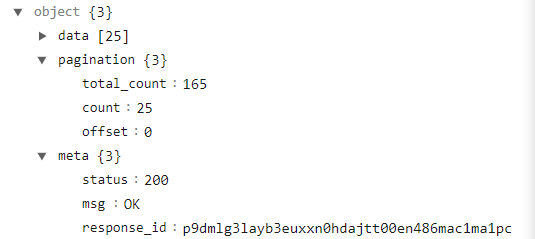
\includegraphics[width=.9\linewidth]{./pic/readme_20221128_194628.png}
\begin{itemize}
\item 从上面的网络反应来看,我的设计太简单了,它可能最外层还需要嵌套androidx jetpack family paging之类相关的东西?需要网上查确认一下
\item 我觉得我不要把这个地方想得太复杂了,它更多的应该是说它网络服务器里的内容很多,能够返回给用户的就是这些而已.而我应该就是把这些显示到recyclerview里就可以了,我应该可以暂时不用考虑paging 相关的.
\item 但是现在能够拿到网络返回结果,需要把网络数据解析好,真正加载出来
\item 晚一点儿再来看这个东西,先把现在已有的设计运行好
\item ● Requirements:
\begin{itemize}
\item Display List of the results.
\end{itemize}
\item ● Results should display:
\begin{itemize}
\item ○ GIFs
\item ○ headline text
\end{itemize}
\end{itemize}
\subsection{Summary:}
\label{sec-2-2}
\begin{itemize}
\item ● Please write code that you feel proud of and would check in to
\begin{itemize}
\item source control or send it to recruiter. Kotlin is preferred.
\end{itemize}
\item ● Please be thorough in your implementation details.
\item ● Please focus on App Architecture and android best practices.
\item ● Bonus points:
\begin{itemize}
\item ○ Implementing application using logical components
\item ○ Unit test coverage
\item ○ Finish project quickly is a plus
\end{itemize}
\end{itemize}
% Emacs 27.2 (Org mode 8.2.7c)
\end{document}